
\documentclass{article}
\usepackage{amsmath}
\usepackage{graphicx}

\begin{document}

\begin{titlepage}
  \centering
  \vspace*{2cm}
  {\Huge\bfseries Report\par}
  \vspace{2cm}
  {\Large\itshape Homework 1\par}
  \vspace{0.5cm}
  {\large\itshape Goal: Develop models for 10-class classification problems with medium and large input space\par}
  \vfill
  {\Large Andrea Massignan\par}
  {\Large 1796802\par}
  \vfill
  {\large\today\par}
\end{titlepage}

\section*{Project Overview}

The goal is to provide two different solution for a 10-class classification problem.

\section{Dataset}

The datasets used in this project consists in training sets and blind test sets.
The training sets are composed by 50000 samples, each one with 100 features for Dataset 1 and 1000 features for Dataset 2.
The blind test sets are composed by 10000 samples, each one with 100 features for Dataset 1 and 1000 features for Dataset 2.
The labels are 10, one for each class.

\begin{itemize}
  \item \texttt{X\_train}: 50000 samples for each dataset.
  \item \texttt{n\_features}: 100 for Dataset 1 and 1000 for Dataset 2.

\end{itemize}

\section{Data Exploration}
The datasets, that are in a csv file, the elements $V^{(i)}$ belonging
to the $X$ column are feature vectors that represent the input data.
\newline
\newline
The Y column contains the associated labels $C_k$(k=0,...9).
\newline
\newline
Thus, each line i in column X is a feature vector structured as:
\newline
\newline
[$V^{(i)}_1$, $V^{(i)}_2$, ..., $V^{(i)}_j$, ... , $V^{(i)}_d$]
\newline
\newline
Where d is the size of the feature vector with sizes described before.
\newline
\newline
And $i=1,...,n$, where n is the number of samples in the dataset as specified before.
\newline
\newline
These are loaded with an helper function called \texttt{load\_data} that returns the training set in the X matrix and the labels in the Y vector.
\newline
\newline
Then the training set is split into \texttt{X\_train} and \texttt{Y\_train} with a test size of $0.2$ and different random states.
\newline
\newline
Since the dataset is already vectorized, no further preprocessing is needed at the moment.

\section{Metrics}
The metrics used to evaluate the models are the accuracy and the confusion matrix.
\newline

\subsection{Precision}
Precision is a measure of the accuracy of the positive predictions made by a model. It is the ratio of true positive predictions to the total number of positive predictions made by the model (both true positives and false positives). Precision is calculated using the formula:
\[
  \text{Precision} = \frac{\text{True Positives}}{\text{True Positives + False Positives}}
\]
Precision provides insight into the model's ability to avoid making false positive predictions. A high precision indicates that when the model predicts a positive class, it is likely to be correct.

\subsection{Recall (Sensitivity or True Positive Rate)}
Recall measures the ability of a model to correctly identify all relevant instances of the positive class. It is the ratio of true positive predictions to the total number of actual positive instances in the dataset (including both true positives and false negatives). Recall is calculated using the formula:
\[
  \text{Recall} = \frac{\text{True Positives}}{\text{True Positives + False Negatives}}
\]
Recall is especially important when the cost of false negatives (missing a positive instance) is high, as it focuses on minimizing false negatives.

\subsection{F1-Score}
The F1-score is the harmonic mean of precision and recall. It provides a balanced measure that considers both false positives and false negatives. The F1-score is calculated using the formula:
\[
  \text{F1-Score} = \frac{2 \times \text{Precision} \times \text{Recall}}{\text{Precision + Recall}}
\]
F1-score is useful when there is an uneven class distribution or when false positives and false negatives have different consequences.

\subsection{Support}
Support refers to the number of actual instances of each class in the dataset. It is the count of true positive and true negative instances for each class. Support is not directly involved in the calculation of precision, recall, or F1-score, but it provides context by showing how many instances belong to each class.

\begin{titlepage}
  \begin{center}
    {\Huge\bfseries Classification\par}
  \end{center}
  \vspace{2cm}

  \section{Data Loading and Splitting}

  \subsection{Loading Dataset 1}
  The data loading process begins with dataset 1, where the feature matrix \(X\) and label vector \(Y\) are extracted using the \texttt{load\_data} function. An informative message is printed to indicate the commencement of this operation. The resulting shape of matrix \(X\) is then presented, providing insights into the number of samples and features within dataset 1.

  \subsection{Loading Dataset 2}
  An analogous procedure is employed for dataset 2. The feature matrix \(X2\) and label vector \(Y2\) are obtained through the \texttt{load\_data} function. A corresponding message is printed, and the shape of \(X2\) is displayed to convey the dataset's sample and feature dimensions.

  \subsection{Splitting Data}
  The subsequent steps involve splitting the loaded data into training and testing sets:

  \begin{verbatim}
  X_train1, X_test1, Y_train1, Y_test1 = train_test_split(X, Y, ...)
    ...
  X_train4, X_test4, Y_train4, Y_test4 = train_test_split(X2, Y2, ...)
  \end{verbatim}

  Utilizing the \texttt{train\_test\_split} function, both dataset 1 and dataset 2 are partitioned into training and testing sets. Each dataset undergoes this process twice, resulting in four sets per dataset.
  The \texttt{test\_size} parameter dictates the proportion allocated for testing (20\%), while \texttt{random\_state} ensures reproducibility.
  \newline
  \newline
  The code concludes by acknowledging the completion of data loading and splitting.
  \newline
  \newline
  The resulting variables (\(X\_train1\), \(X\_test1\), \(Y\_train1\), \(Y\_test1\), etc.) are now ready for subsequent machine learning tasks.

\end{titlepage}

\begin{titlepage}
  \section*{Model Selection}
  After the data is loaded and splitted, the user is prompted to choose which of the dataset to use and then what type of model to use for the classification task. The user can choose between:
  \section{Bernoulli}
  BernoulliNB is a Naive Bayes classifier specifically tailored for multivariate Bernoulli models. Similar to MultinomialNB, this classifier is well-suited for handling discrete data.
  \newline
  \newline
  The key distinction lies in their data types:
  MultinomialNB deals with occurrence counts, while BernoulliNB is optimized for binary or boolean features.
  BernoulliNB is preferred over other Naive Bayes classifiers when dealing with datasets where features are binary or boolean.
  \newline
  \newline
  It is well-suited for problems involving discrete, binary decision-making based on the presence or absence of features.
  Additionally, BernoulliNB is a simpler model with fewer parameters, making it advantageous for scenarios with limited training data and leading to faster training and prediction times.

  \subsection{Classification}
  Overall the model performs well, with an average accuracy of 90\%, however class 3 has a lower recall of 71\%, meaning that the model struggles to capture all instances of the class.
  \newline
  \newline
  Even class 4 has a lower precision of 78\%, meaning that when the model predicts this class it's not always correct.

  \begin{figure}[htbp]
    \centering
    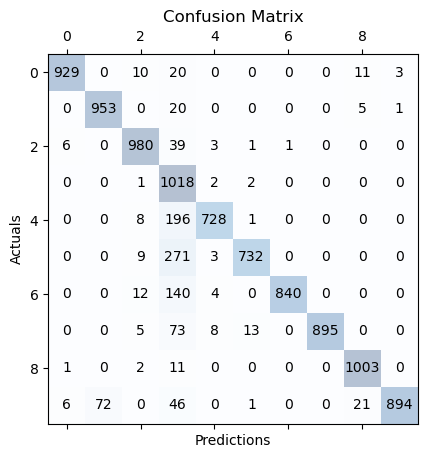
\includegraphics[width=0.4\textwidth]{bernoulliCM.png}
    \caption{Confusion Matrix for BernoulliNB}
    \label{fig:sample}
  \end{figure}

  \section{SVM}
  Support Vector Machine is a supervised machine learning algorithm used for classification and regression tasks. It's particularly powerful in high-dimensional spaces and is effective in cases where the margin between different classes is clear.
  \newline
  \newline
  The SVM model performs well in terms of precision and recall for most classes, but there are variations across different digits.
  \newline
  In this particular case we are using a linear kernel, which is a good choice for high-dimensional data, however, it may not be the best choice for this particular dataset.

  \begin{itemize}
    \item The accuracy is around 83\% which is lower than the BernoulliNB model.
    \item Some classes, like class 5, have lower support (973), while others, like class 7, have higher support (1048).
    \item The F1-scores are generally high, however, class 2 stands out with a lower F1-score (0.22).
    \item Notably, class 5 has a recall of 1.00, on the other hand, classes 2 and 3 have lower recall values.
    \item For most classes, precision is relatively high, however, there are exceptions, such as class 5, where precision is notably lower (0.40).
  \end{itemize}

  The lower performance in certain classes, especially in terms of recall for classes 2 and 3, indicates areas where the model may benefit from further improvement.

  \begin{figure}[htbp]
    \centering
    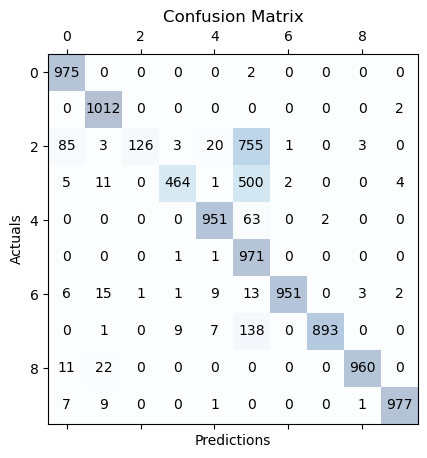
\includegraphics[width=0.5\textwidth]{SVMCM.png}
    \caption{Confusion Matrix for SVM}
    \label{fig:sample2}
  \end{figure}

\end{titlepage}


\end{document}
